

\tikzset{every picture/.style={line width=0.75pt}} %set default line width to 0.75pt        

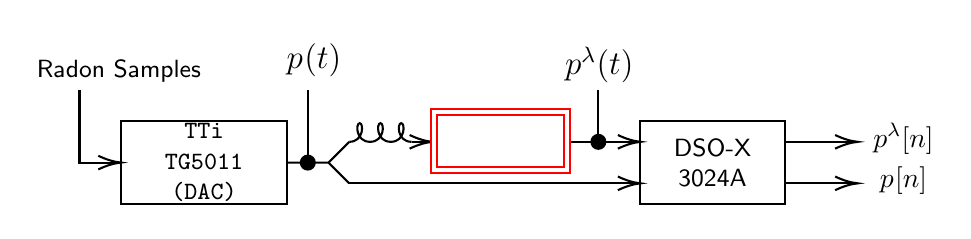
\begin{tikzpicture}[x=0.75pt,y=0.75pt,yscale=-1,xscale=1]
%uncomment if require: \path (0,100); %set diagram left start at 0, and has height of 100

%Shape: Rectangle [id:dp4535952511777318] 
\draw   (60,50) -- (140,50) -- (140,90) -- (60,90) -- cycle ;
%Shape: Spring [id:dp24973351992992] 
\draw   (200,60) .. controls (193,60) and (193,51) .. (195,51) .. controls (197,51) and (197,60) .. (190,60) .. controls (183,60) and (183,51) .. (185,51) .. controls (187,51) and (187,60) .. (180,60) .. controls (173,60) and (173,51) .. (175,51) .. controls (177,51) and (177,60) .. (170,60) ;
%Straight Lines [id:da5443117852195816] 
\draw    (58,70) -- (40,70) -- (40,35) ;
\draw [shift={(60,70)}, rotate = 180] [color={rgb, 255:red, 0; green, 0; blue, 0 }  ][line width=0.75]    (10.93,-3.29) .. controls (6.95,-1.4) and (3.31,-0.3) .. (0,0) .. controls (3.31,0.3) and (6.95,1.4) .. (10.93,3.29)   ;
%Shape: Rectangle [id:dp7033377008796209] 
\draw   (310,50) -- (380,50) -- (380,90) -- (310,90) -- cycle ;
%Straight Lines [id:da35471550888079884] 
\draw    (170,80) -- (308.33,80) ;
\draw [shift={(310.33,80)}, rotate = 180] [color={rgb, 255:red, 0; green, 0; blue, 0 }  ][line width=0.75]    (10.93,-3.29) .. controls (6.95,-1.4) and (3.31,-0.3) .. (0,0) .. controls (3.31,0.3) and (6.95,1.4) .. (10.93,3.29)   ;
%Straight Lines [id:da8899034724605472] 
\draw    (210,60) -- (308.33,60) ;
\draw [shift={(310.33,60)}, rotate = 180] [color={rgb, 255:red, 0; green, 0; blue, 0 }  ][line width=0.75]    (10.93,-3.29) .. controls (6.95,-1.4) and (3.31,-0.3) .. (0,0) .. controls (3.31,0.3) and (6.95,1.4) .. (10.93,3.29)   ;
%Straight Lines [id:da9241889627132005] 
\draw    (140,70) -- (160,70) -- (170,60) ;
%Straight Lines [id:da6785042681502754] 
\draw    (160,70) -- (170,80) ;
%Straight Lines [id:da8399866894570822] 
\draw    (200,60) -- (208,60) ;
\draw [shift={(210,60)}, rotate = 180] [color={rgb, 255:red, 0; green, 0; blue, 0 }  ][line width=0.75]    (10.93,-3.29) .. controls (6.95,-1.4) and (3.31,-0.3) .. (0,0) .. controls (3.31,0.3) and (6.95,1.4) .. (10.93,3.29)   ;
%Straight Lines [id:da3291742157799078] 
\draw    (150,70) -- (150,35) ;
\draw [shift={(150,70)}, rotate = 270] [color={rgb, 255:red, 0; green, 0; blue, 0 }  ][fill={rgb, 255:red, 0; green, 0; blue, 0 }  ][line width=0.75]      (0, 0) circle [x radius= 3.35, y radius= 3.35]   ;
%Straight Lines [id:da4267771870696746] 
\draw    (290,60) -- (290,35) ;
\draw [shift={(290,60)}, rotate = 270] [color={rgb, 255:red, 0; green, 0; blue, 0 }  ][fill={rgb, 255:red, 0; green, 0; blue, 0 }  ][line width=0.75]      (0, 0) circle [x radius= 3.35, y radius= 3.35]   ;
%Straight Lines [id:da7428870484261483] 
\draw    (380,60) -- (413,60) ;
\draw [shift={(415,60)}, rotate = 180] [color={rgb, 255:red, 0; green, 0; blue, 0 }  ][line width=0.75]    (10.93,-3.29) .. controls (6.95,-1.4) and (3.31,-0.3) .. (0,0) .. controls (3.31,0.3) and (6.95,1.4) .. (10.93,3.29)   ;
%Straight Lines [id:da7684449384615536] 
\draw    (380,80) -- (413,80) ;
\draw [shift={(415,80)}, rotate = 180] [color={rgb, 255:red, 0; green, 0; blue, 0 }  ][line width=0.75]    (10.93,-3.29) .. controls (6.95,-1.4) and (3.31,-0.3) .. (0,0) .. controls (3.31,0.3) and (6.95,1.4) .. (10.93,3.29)   ;

% Text Node
\draw (100,70) node  [font=\small] [align=left] {\begin{minipage}[lt]{45.85pt}\setlength\topsep{0pt}
\begin{center}
{\texttt{TTi TG5011}}\\{\texttt{(DAC)}}
\end{center}

\end{minipage}};
% Text Node
\draw (345,70) node  [font=\small] [align=left] {\begin{minipage}[lt]{31.79pt}\setlength\topsep{0pt}
\begin{center}
\sf{DSO-X}\\\sf{3024A}
\end{center}

\end{minipage}};
% Text Node
\draw (153,20.5) node  [font=\large]  {$p_{\bftheta }( t)$};
% Text Node
\draw (437,58.5) node  [font=\normalsize]  {$p_{\bftheta }^{\lambda }[ n]$};
% Text Node
\draw (437,78.5) node  [font=\normalsize]  {$p_{\bftheta }[ n]$};
% Text Node
\draw (59,26) node  [font=\small] [align=left] {\sf{Radon Samples}};
% Text Node
\draw  [draw opacity=0]  (265.5,5.5) -- (315.5,5.5) -- (315.5,40.5) -- (265.5,40.5) -- cycle  ;
\draw (290.5,23) node  [font=\large] [align=left] {$p_{\bftheta }^{\lambda }( t)$};
% Text Node
\draw  [color={rgb, 255:red, 255; green, 0; blue, 0 }  ,draw opacity=1 ][fill={rgb, 255:red, 255; green, 255; blue, 255 }  ,fill opacity=1 ]  (212.38,47) -- (273.38,47) -- (273.38,72) -- (212.38,72) -- cycle (209.38,44) -- (276.38,44) -- (276.38,75) -- (209.38,75) -- cycle ;
\draw (242.88,59.5) node   [align=left] { \ \madc \ };


\end{tikzpicture}
